\documentclass{sigchi}

% Use this section to set the ACM copyright statement (e.g. for
% preprints).  Consult the conference website for the camera-ready
% copyright statement.

% Copyright
\CopyrightYear{2016}
%\setcopyright{acmcopyright}
\setcopyright{acmlicensed}
%\setcopyright{rightsretained}
%\setcopyright{usgov}
%\setcopyright{usgovmixed}
%\setcopyright{cagov}
%\setcopyright{cagovmixed}
% DOI
\doi{http://dx.doi.org/10.475/123_4}
% ISBN
\isbn{123-4567-24-567/08/06}
%Conference
\conferenceinfo{CHI'16,}{May 07--12, 2016, San Jose, CA, USA}
%Price
\acmPrice{\$15.00}

% Use this command to override the default ACM copyright statement
% (e.g. for preprints).  Consult the conference website for the
% camera-ready copyright statement.

%% HOW TO OVERRIDE THE DEFAULT COPYRIGHT STRIP --
%% Please note you need to make sure the copy for your specific
%% license is used here!
% \toappear{
% Permission to make digital or hard copies of all or part of this work
% for personal or classroom use is granted without fee provided that
% copies are not made or distributed for profit or commercial advantage
% and that copies bear this notice and the full citation on the first
% page. Copyrights for components of this work owned by others than ACM
% must be honored. Abstracting with credit is permitted. To copy
% otherwise, or republish, to post on servers or to redistribute to
% lists, requires prior specific permission and/or a fee. Request
% permissions from \href{mailto:Permissions@acm.org}{Permissions@acm.org}. \\
% \emph{CHI '16},  May 07--12, 2016, San Jose, CA, USA \\
% ACM xxx-x-xxxx-xxxx-x/xx/xx\ldots \$15.00 \\
% DOI: \url{http://dx.doi.org/xx.xxxx/xxxxxxx.xxxxxxx}
% }

% Arabic page numbers for submission.  Remove this line to eliminate
% page numbers for the camera ready copy
% \pagenumbering{arabic}

% Load basic packages
\usepackage{balance}       % to better equalize the last page
\usepackage{graphics}      % for EPS, load graphicx instead 
\usepackage[T1]{fontenc}   % for umlauts and other diaeresis
\usepackage{txfonts}
\usepackage{mathptmx}
\usepackage[pdflang={en-US},pdftex]{hyperref}
\usepackage{color}
\usepackage{booktabs}
\usepackage{textcomp}

% Some optional stuff you might like/need.
\usepackage{microtype}        % Improved Tracking and Kerning
% \usepackage[all]{hypcap}    % Fixes bug in hyperref caption linking
\usepackage{ccicons}          % Cite your images correctly!
% \usepackage[utf8]{inputenc} % for a UTF8 editor only

% If you want to use todo notes, marginpars etc. during creation of
% your draft document, you have to enable the "chi_draft" option for
% the document class. To do this, change the very first line to:
% "\documentclass[chi_draft]{sigchi}". You can then place todo notes
% by using the "\todo{...}"  command. Make sure to disable the draft
% option again before submitting your final document.
\usepackage{todonotes}

% Paper metadata (use plain text, for PDF inclusion and later
% re-using, if desired).  Use \emtpyauthor when submitting for review
% so you remain anonymous.
\def\plaintitle{SIGCHI Conference Proceedings Format}
\def\plainauthor{First Author, Second Author, Third Author,
  Fourth Author, Fifth Author, Sixth Author}
\def\emptyauthor{}
\def\plainkeywords{Authors' choice; of terms; separated; by
  semicolons; include commas, within terms only; required.}
\def\plaingeneralterms{Documentation, Standardization}

% llt: Define a global style for URLs, rather that the default one
\makeatletter
\def\url@leostyle{%
  \@ifundefined{selectfont}{
    \def\UrlFont{\sf}
  }{
    \def\UrlFont{\small\bf\ttfamily}
  }}
\makeatother
\urlstyle{leo}

% To make various LaTeX processors do the right thing with page size.
\def\pprw{8.5in}
\def\pprh{11in}
\special{papersize=\pprw,\pprh}
\setlength{\paperwidth}{\pprw}
\setlength{\paperheight}{\pprh}
\setlength{\pdfpagewidth}{\pprw}
\setlength{\pdfpageheight}{\pprh}

% Make sure hyperref comes last of your loaded packages, to give it a
% fighting chance of not being over-written, since its job is to
% redefine many LaTeX commands.
\definecolor{linkColor}{RGB}{6,125,233}
\hypersetup{%
  pdftitle={\plaintitle},
% Use \plainauthor for final version.
%  pdfauthor={\plainauthor},
  pdfauthor={\emptyauthor},
  pdfkeywords={\plainkeywords},
  pdfdisplaydoctitle=true, % For Accessibility
  bookmarksnumbered,
  pdfstartview={FitH},
  colorlinks,
  citecolor=black,
  filecolor=black,
  linkcolor=black,
  urlcolor=linkColor,
  breaklinks=true,
  hypertexnames=false
}

% create a shortcut to typeset table headings
% \newcommand\tabhead[1]{\small\textbf{#1}}
\newcommand{\interface}[0]{\textit{Our Interface}}

\newcommand {\wil}[1]{{\color{green}\bf{WL: #1}\normalfont}}
\newcommand {\val}[1]{{\color{blue}\bf{VS: #1}\normalfont}}
\newcommand {\fd}[1]{{\color{magenta}\bf{FD: #1}\normalfont}}

% End of preamble. Here it comes the document.
\begin{document}

\title{\plaintitle}

\numberofauthors{3}
\author{%
  \alignauthor{Leave Authors Anonymous\\
    \affaddr{for Submission}\\
    \affaddr{City, Country}\\
    \email{e-mail address}}\\
  \alignauthor{Leave Authors Anonymous\\
    \affaddr{for Submission}\\
    \affaddr{City, Country}\\
    \email{e-mail address}}\\
  \alignauthor{Leave Authors Anonymous\\
    \affaddr{for Submission}\\
    \affaddr{City, Country}\\
    \email{e-mail address}}\\
}

\maketitle

\begin{abstract}
  UPDATED---\today. This sample paper describes the formatting
  requirements for SIGCHI conference proceedings, and offers
  recommendations on writing for the worldwide SIGCHI
  readership. Please review this document even if you have submitted
  to SIGCHI conferences before, as some format details have changed
  relative to previous years. Abstracts should be about 150 words and
  are required.
\end{abstract}

\category{H.5.m.}{Information Interfaces and Presentation
  (e.g. HCI)}{Miscellaneous} \category{See
  \url{http://acm.org/about/class/1998/} for the full list of ACM
  classifiers. This section is required.}{}{}

\keywords{\plainkeywords}
\section{Introduction}

Presentation technology has a significant impact on how we learn and teach. Today, there are largely two modes of presentation technology used in classrooms: inking on surface and projecting prepared slides. \\
35mm slide projectors first came into widespread use during the 1950s, but recently the popularization of slide authoring tools like PowerPoint, Keynote or Google Slides made electronic slides became much more common and easy. Despite its advantages--e.g., easy to share, archive, include multimedia--slides also have critical drawbacks. 
(1) Slide presentations are \textbf{rigid}: All of the editing and preparation is done ahead of time and fixed at the time of the presentation. There is no flexibility to change the order or content of the presentation during performance. 
(2) Slide presentations are \textbf{discrete}: Information is divided and presented in chunks. First the entire content is divided into separate slides, and within each slide text or graphics are presented in chunks, usually using animation effects. The appearance or transition of information is sudden and discrete.
(3) Slide presentations are \textbf{indirect}: The action of the presenter (i.e., pressing "next" to advance the slide) is removed from the effect on the content. For example, this makes it easy for presenters to forget or skip an animation sequence.\\

Inking on surface is an alternative or supplement. Inking includes blackboard or transparency and overhead projector. Inking complements the characteristics of slides. Inking is flexible, continuous and direct, but this has its own downsides.
(1) Inking is \textbf{flexible} since all of the presentation is done on the fly. But, this means there is a lot of cognitive overload for the presenter in order to decide the content, layout and order of the presentation on the fly. 
(2) Inking is \textbf{continuous}: Since the presenter writes or draws in real time, content is presented in a continuous way. This is useful for information-loaded contents or where order within the content is important, for example, derivation of a math formula or describing a temporal process. However, it is difficult to time the presentation or present a lot of information. Inking lectures tend to be slower paced [citation].
Finally, (3) inking is direct. Users actions (drawing, erasing, underlying) are all directly translated into content. This requires a lot of attention, skill on the part of the presenter. Often, presenters are reluctant to write because of their messy handwriting. Also content is limited to text or simple diagrams.

There are previous work to blend the two modes. [Classroom Presenter] or recent versions of [PowerPoint] allow you to ink on slides. But these tools treat the two modes as separate. Ink and slide remain separate layers retaining their characteristics. The slide layer remains rigid and fixed; and ink is placed on top of it.

\textbf{We propose inking as a main modality to present slide contents in a continuous, flexible and direct manner}. By inking over to reveal content, users regain flexibility, continuity and direct control over the presentation style, without losing the elegance of the prepared content.  


\section{Related Work}

\textbf{Presentation Software.} The vast majority of presentations today are created with WYSIWYG slide authoring software like PowerPoint \cite{powerpoint2017}, Keynote \cite{keynote2017} and Google Slides \cite{googleslides2017}. 
%
While these tools provide a broad range of content creation features, including the ability to add animation effects to slide elements, 
they offer limited flexibility or control at presentation time. 
%
Presenters can only advance linearly through the predefined sequence of animations and slide transitions.

\textbf{Nonlinear Presentations.} To address this shortcoming, previous research investigates how to support nonlinear paths though a presentation. Moscovich et al \cite{moscovich2004customizable} organize slides into nested directed graphs and allow presenters to choose between multiple paths on the fly. Similarly, Drucker et al. \cite{drucker2006comparing} suggest a method to compare and manage multiple slide presentation paths. Fly \cite{lichtschlag2009fly} and CounterPoint \cite{good2002zoomable} allow spatial navigation by embedding slides on an infinite canvas and employing zooming user interfaces (ZUIs). Prezi \cite{prezi2017} is a commercial, online platform for authoring zoomable presentations. Whereas this work focuses on navigating between slides or the presentation as a whole, the interactions in our work provide flexibility and control within each slide.

\textbf{Controlling Presentations.} Other work explores alternative techniques to control slide presentations. Palette \cite{nelson1999palette} uses physical cards to provide random access to slides, Baudel and Beaudouin-Lafon \cite{baudel1993charade} propose hand gestures, and Cheng and Pulo \cite{cheng2003direct} use an infrared laser pointer to control presentations. Cao et al. \cite{cao2005evaluation} perform a systematic user study comparing different interaction techniques, including hand gestures, laser pointer and standard mouse/keyboard input. Our work suggests inking interactions as the main mode to present slides.

\textbf{Inking on Digital Documents.} Many systems \cite{yoon2014richreview, marshall1999collaborating, hardock1993marking} support digital inking to make annotations on top of documents. Perhaps most similar in spirit to our work are systems that integrate digital ink with prepared slides. Anderson et al.~\cite{anderson2007classroom} propose Classroom Presenter, a distributed presentation system that allows instructors and students to share digital ink on top of electronic slides. Recently, PowerPoint and Keynote added support for presenters to ink in presentation mode as well. SMART is another commercial system that supports inking and projected material using an interactive whiteboard \cite{smarttech2017}. While all of these systems combine slides with inking, the underlying slide content remains inherently separate from the ink on top. In contrast, in our system, presenters use ink to reveal underlying slide elements in a flexible, fine-grained way at presentation time.
%\val{This sentence would also benefit from clarification of inking: as a gesture vs. output.} 
%\wil{Is that better?}

\textbf{Beautifying Ink.} To further assist freeform digital inking, researchers have experimented with different methods to beautify the user's ink strokes. Beautification is applied to meet the requirements of specific scenarios, such as geometric diagrams \cite{igarashi1998pegasus, hse2005recognition, fivser2015shipshape}, hand-drawn pictures~\cite{xie2014portraitsketch, limpaecher2013}, handwriting \cite{zitnick2013handwriting} or mathematical diagrams~\cite{laviola2007mathpad}. Our work does not modify the user's ink stroke per se, but we achieve a similar effect by making the ink stroke disappear gradually and revealing the underlying pre-authored slide content instead.

\section{Current Practice and Needs}
To learn about current practice and unsupported needs in presentation technology, we conducted multiple rounds of interviews with classroom lecturers, online lecturers, graduate student TAs, and undergraduate students, with varied experiences in giving and listening to presentations. 
%
We also consulted existing literature comparing different types of presentation software.
%
From this analysis, we summarize the key findings that informed the design of our system.

\textbf{Flexibility in presentations is preferred for interactive or informal settings.} For settings such as research conferences or business meetings with tight time constraints and little room for audience interaction, people prefer to give highly scripted presentations with electronic slides. However, for settings such as lectures, tutoring sessions, or brainstorming meetings, presenters like to have some flexibility and often use inking as part of their presentations. Common strategies include using a blackboard or projecting slides/transparencies onto a board and inking on top of them. Several lecturers purposefully leave blank spaces on their slides to fill in by inking during the lecture. %Inking allows presenters to draw attention to content by writing or annotating in real time, to modify the order in which content is presented, or in some cases, to modify the content itself based on audience input or feedback.

\textbf{Presenters want flexibility over prepared contents rather than complete improvisation.} Even for informal settings, presenters have the bulk of the content planned and prepared beforehand, in the form of lecture notes, worksheets or slides. Thus, the type of flexibility that presenters want is the ability to make small-scale adjustments on-the-fly, such as omitting part of the content, adding minor changes such as a line of text or annotations, or changing the order of the contents. Inking is often used to this effect. 
%\wil{This is repetitive with the last sentence in the previous paragraph.}

\textbf{Pacing is important and context dependent.} 
The choice of tool also affects the pace of the presentation. Electronic slides are useful for displaying information quickly, which may explain why presenters prefer them for time-constrained settings. Inking takes time, but it allows presenters to have fine-grained control over the pace of the presentation. Depending on the subject matter, the pace of real time writing also makes it easier to follow for the audience. For example, when describing sequential processes like solving a math problem or explaining a complex diagram, both presenters and viewers find it more effective to write them out step-by-step in real-time. Slide animations can simulate this effect, but setting up fine-grained animations is tedious. As a result, animated presentations typically include a very coarse set of discrete steps. 

\textbf{Visual aesthetics matter but are difficult to achieve with inking.} Both as a presenter and as an audience, people frequently mentioned better visual aesthetics as an advantage of slides over inking. Presenters are often not satisfied with or even embarrassed by their own handwriting. They pointed out that it is even more difficult to write while talking at the same time. Even small operations, such as changing the pen color, seem burdensome during the lecture, as noted by Anderson\cite{anderson2004study}. 
% \wil{Previous two sentences don't seem to be about aesthetics. Is there a separate observation to make about timing? Or could this go into the first observation on context-dependent flexibility?}
%
From a viewing perspective, people like the legibility and organization that pre-authored slides provide. As \cite{frey2002learners} also mention, sometimes audiences even felt that lecturers are better prepared when they present using electronic slides. 
%\wil{For the two points with citations, are these things that also came up in your interviews, or are you just citing previous findings? If the former, we should try to make that clear, as I did with the Anderson reference above.}
\begin{figure*}[t!]
    \centering
    \begin{subfigure}[t]{0.32\textwidth}
        \centering
        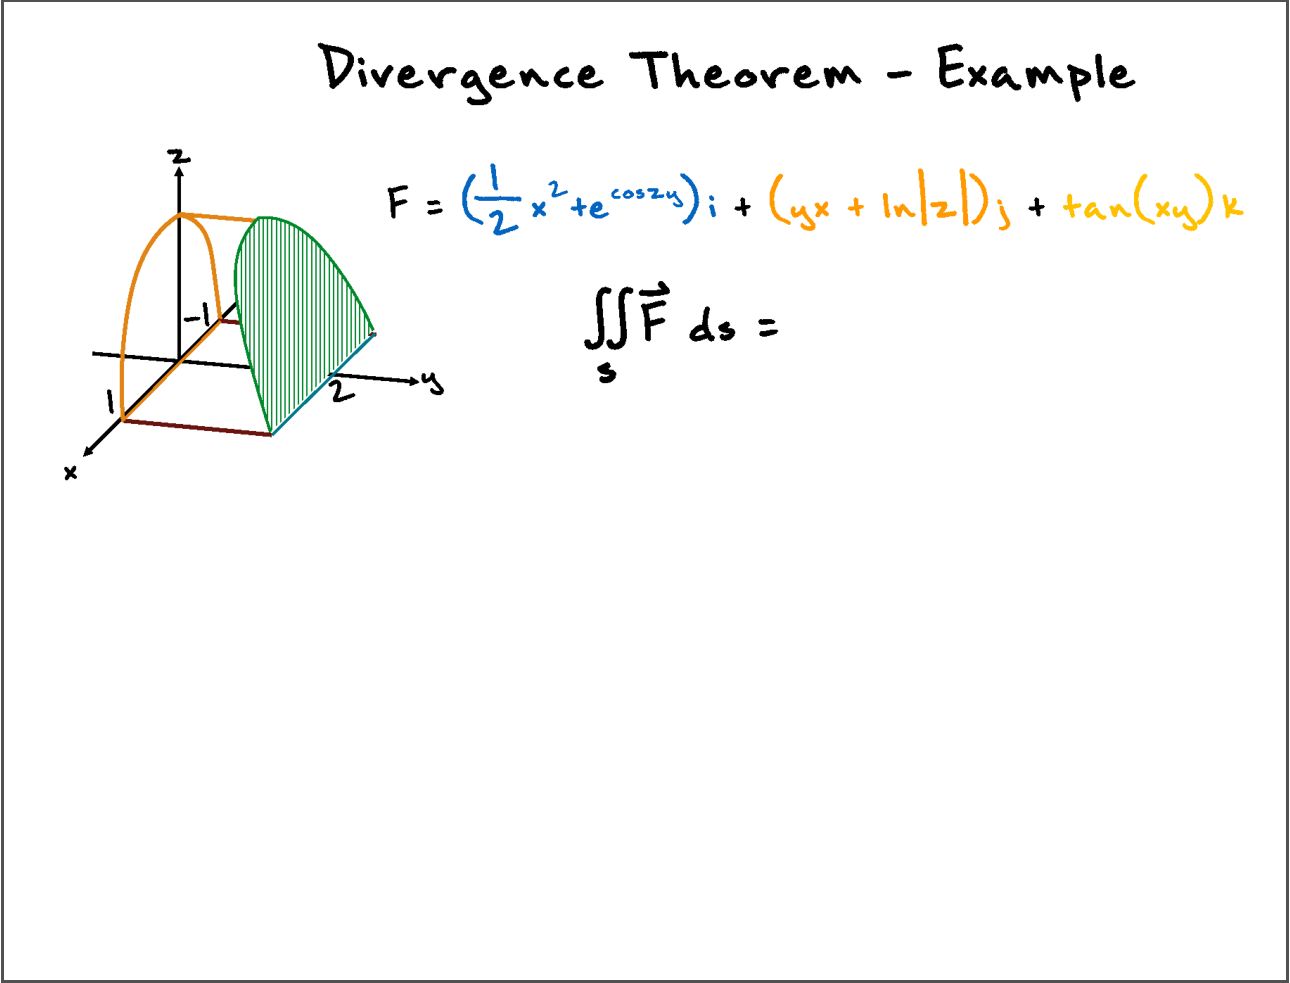
\includegraphics[width=1\columnwidth]{figures/videoslide1}
        \caption{Background (Audience View)}
    \end{subfigure}%
    ~ 
    \begin{subfigure}[t]{0.32\textwidth}
        \centering
        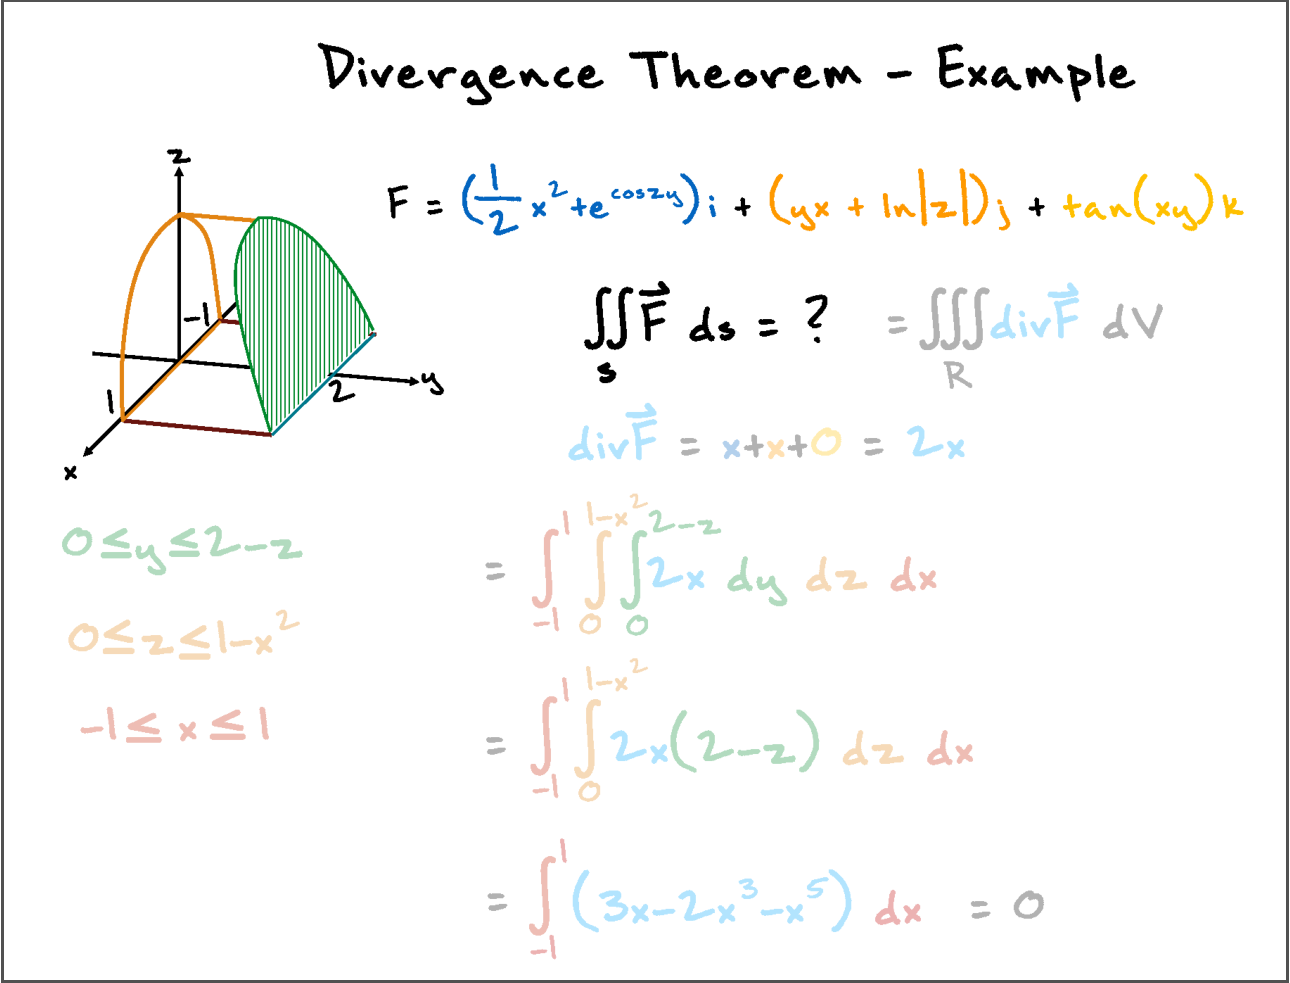
\includegraphics[width=1\columnwidth]{figures/videoslide2}
        \caption{Background + Foreground (Presenter View)}
    \end{subfigure}
    ~
        \begin{subfigure}[t]{0.32\textwidth}
        \centering
        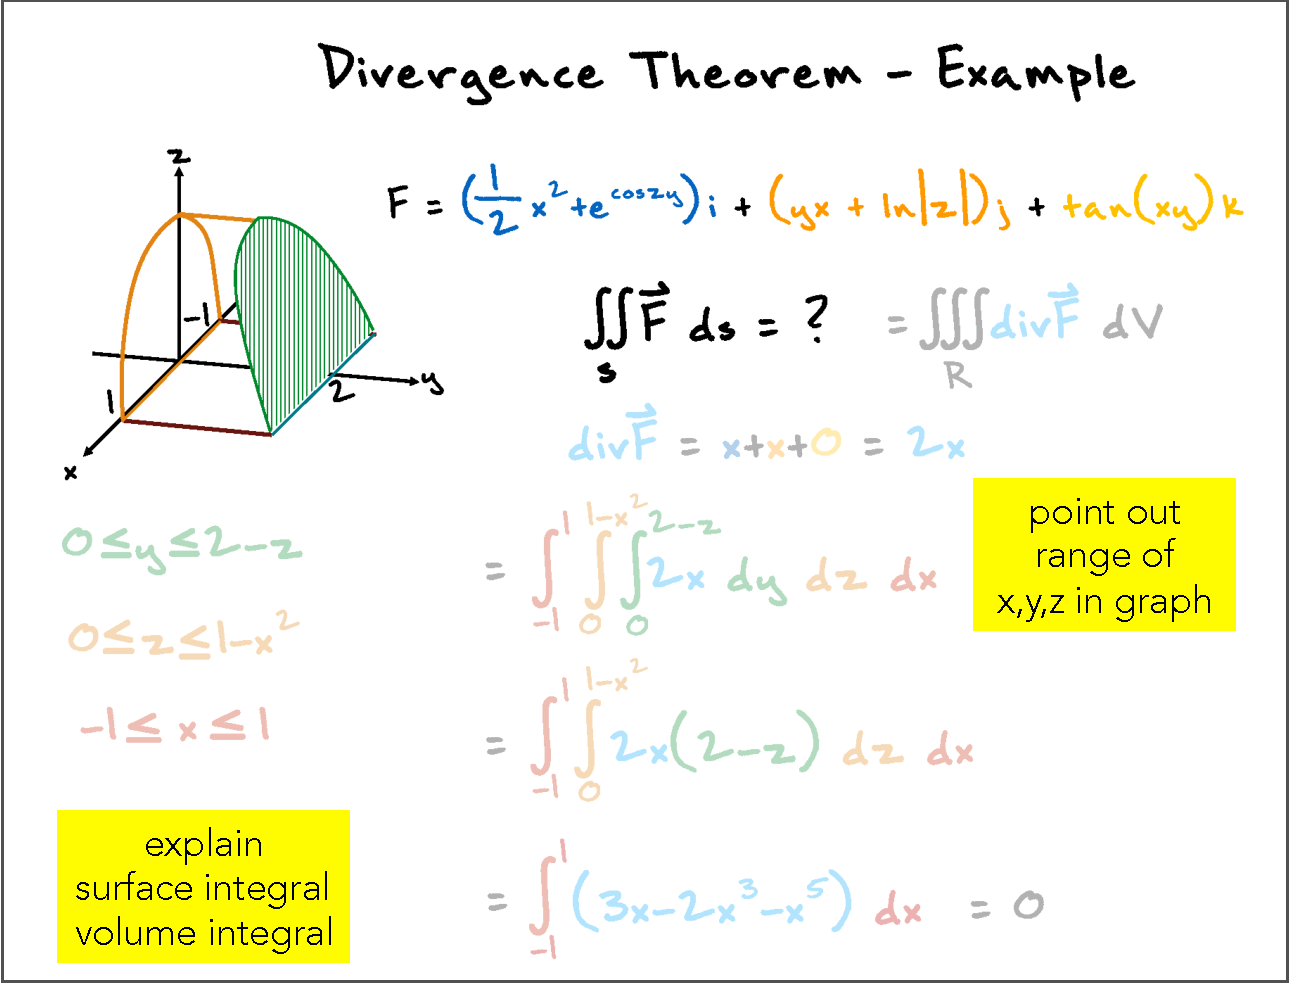
\includegraphics[width=1\columnwidth]{figures/videoslide3}
        \caption{Background + Foreground + Notes}
    \end{subfigure}
    \caption{Slide Layers in \interface. Slides are separated into foreground and background layers. \textbf{(a)} The background layer is always visible and it is what the audience sees initially. \textbf{(b)} The foreground layer is initially only visible on the presenter view, and is faded to distinguish it from the background. Presenters can reveal parts of it to the audience during delivery. The revealed parts appear on the audience view and becomes unfaded on the presenter view. \textbf{(c)} Optionally, presenters can also have the notes layer, which is only visible on the presenter view and acts as transparent speaker notes placed on top of the slides. }
    \label{fig:slidelayers}
\end{figure*}
\section{Design Goals}

The above findings highlight the complementary attributes of electronic slides and inking. While slides are typically more organized and aesthetically pleasing, inking offers greater flexibility and fine-grained control at presentation time.
%
Our aim is to develop a presentation interface that combines the advantages of both existing technologies without increasing the burden on the presenter at authoring and presentation time.
%
More specifically, our system should achieve the following design goals. The first two goals are concerned with improving the presentation quality, while the last goal involves reducing the presenters' effort. 

\textbf{Maximize organization and aesthetics through pre-authored contents.} In order to improve presentation quality, we want to take full advantage of contents that presenters prepare beforehand. Pre-authored contents can help achieve visual aesthetics. It also \textit{forces} the presenter to organize the presentation ahead of time. 
 
\textbf{Maximize flexibility and fine-grained control during presentation delivery.} Presenters should have fine control over what visual content to present, and also when, how much, and how fast to present them. Moreover, these decisions need not be made ahead of time; instead, presenters should be able to implement and adjust them while delivering, according to the content and audience. 

\textbf{Minimize presenter effort during delivery as well as during preparation.} We want to give presenters more control, but without increasing their burden. Interactions during delivery should be as simple and natural as possible. Similarly, preparation itself should not take more effort than, for example, authoring regular slides. Moreover, presenters should be allowed to focus more on preparing the content itself rather than, for instance, spending time to setup animations effects for delivery. 

%These design goals are expressed in \interface in the following ways. 



\section{Design of \interface}
\wil{Before getting into the details of the method, I think we should
  describe the key aspects of our design (fine-grained reveal and
  space manipulation, right?) and connect them to our design principles.}

\interface uses pre-authored slides, prepared by the presenters ahead of time, in pretty much the same way as they would for a regular electronic presentation. The slides help presenters organize their material and to improve visual aesthetics. However, unlike traditional electronic slides, presenters do not specify beforehand when, how, or in which order the elements in the slide will appear (i.e., animation effects). Instead, they simply specify which elements will be displayed to the audience immediately versus which elements will be revealed in real time. 

\interface's main mode of interaction during delivery is inking. Inking has three functions depending on the context: it can (1) reveal pre-authored slide elements to the audience, (2) add ink strokes on top of the slide, or (3) adjust the slide layout by creating blank space. Inking allows presenters to have flexibility and fine-grained control over when, how much, and how fast to reveal elements on the slide. Presenters can also add extra writings or annotations on top of pre-authored elements, and create blank space if necessary. All of these interactions are implemented as modeless pen interactions. 
 
\subsection{Slide authoring}
\val{Figure showing example of background / foreground / notes}
Slides in \interface can be authored using any existing slide presentation software (e.g., PowerPoint, Keynote, GoogleSlides). They can include typed text or images, as well as, hand drawn ink strokes. Instead of specifying animation effects on these slide elements, presenters separate them into two layers for each slide. The background layer is always visible and it is what the audience sees initially. The foreground layer is initially only visible on the presenter view, but presenters can reveal parts of it to the audience during delivery. ]\val{Presenters also have the option of preparing a third layer, the notes layer, which is only visible on the presenter view and serves as a transparent lecture note placed on top of the slides.} Layers in \interface are represented as bitmap images. 

\subsection{Inking during delivery}
During delivery, presenters ink on top of the pre-authored slides. Inking has three different functions depending on the context. 
\textbf{Reveal}
If the presenter inks over \val{around? I want to somehow convey that inking over does not have to be precise: i.e. on top of the pixels} foreground pixels that have not been revealed to the audience yet, these and neighboring foreground pixels are revealed to the audience in the following way. For each point, $s_i$ in the user's ink stroke, the closest foreground pixel, $p_i$ is computed. If $p_i$ is close enough to $s_i$, a flood-fill is performed starting from $p_i$ to neighboring foreground pixels. The extent of the flood-fill is limited by thresholds on (1) the distance from $p_i$, and (2) the color difference from $p_i$. In order to give presenters finer-grained control over the extent of the reveal, the thresholds vary according to the velocity of the presenter's ink stroke. If the presenter inks slowly, only a small neighborhood close to the original stroke is revealed. This is useful when the presenter wants to simulate writing in real-time, and reveal, for example, a part of a character or a diagram. If the presenter inks quickly (e.g., scribbles), a larger neighborhood is revealed. This allows presenters, for instance, to swiftly reveal an entire image or a line of text without having to ink over them precisely.  \val{Figure showing user tracing over a formula, one character at a time}

\textbf{Annotate}
If the presenter inks over empty pixels on the foreground, or if the foreground pixels around the stroke has already been revealed previously, the ink stroke appears on top of the foreground layer as is. \interface computes the average color of the slide around the stroke and sets the ink color to a complementary color so that the ink stands out from the slide. \val{Figure of annotation over revealed element and annotation on empty background}. 

\textbf{Create Space}
Sometimes, presenters may want extra space to insert new content in the slide, for example, to add an item to an existing list, a word in a sentence, or an extra line of explanation. These situations can arise as a result of a mistake in the preparation phase (e.g., the presenter forgets to list an item), as well as from presenter-audience interaction (e.g., the audience requests extra explanation). \interface allows presenters to create empty space from ink strokes. First, the presenter draws a curve where the empty space is to be created. At the end of the curve, if the presenter holds down the pen for more than 0.5 seconds, the curve turns into a red dashed stroke, indicating that the presenter can start expanding the space around the curve. As the presenter moves the pen along one of the axis-aligned directions, empty space is created and expanded from the curve in that direction.  As the space grows, the foreground content is shifted accordingly. \val{Figure showing the steps.}

\section{Result}
Emphasize some of the benefits of our tool.
(1) Order of presentation is flexible and does not have to be prepared beforehand. 
(2) Modeless switch between revealing and annotation.

Show and describe some presentations created with our tool.

\section{User Evaluation}
\begin{figure}[t!]
    \centering
    \begin{subfigure}[t]{1\columnwidth}
        \centering
        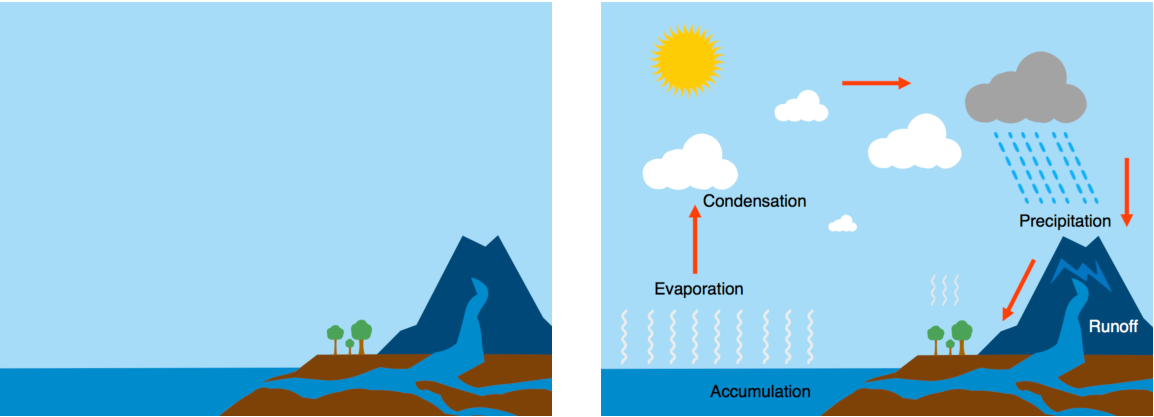
\includegraphics[width=1\columnwidth]{figures/watercycle}
        \caption{Lorem ipsum}
    \end{subfigure}
    ~ 
    \begin{subfigure}[t]{0.48\columnwidth}
        \centering
        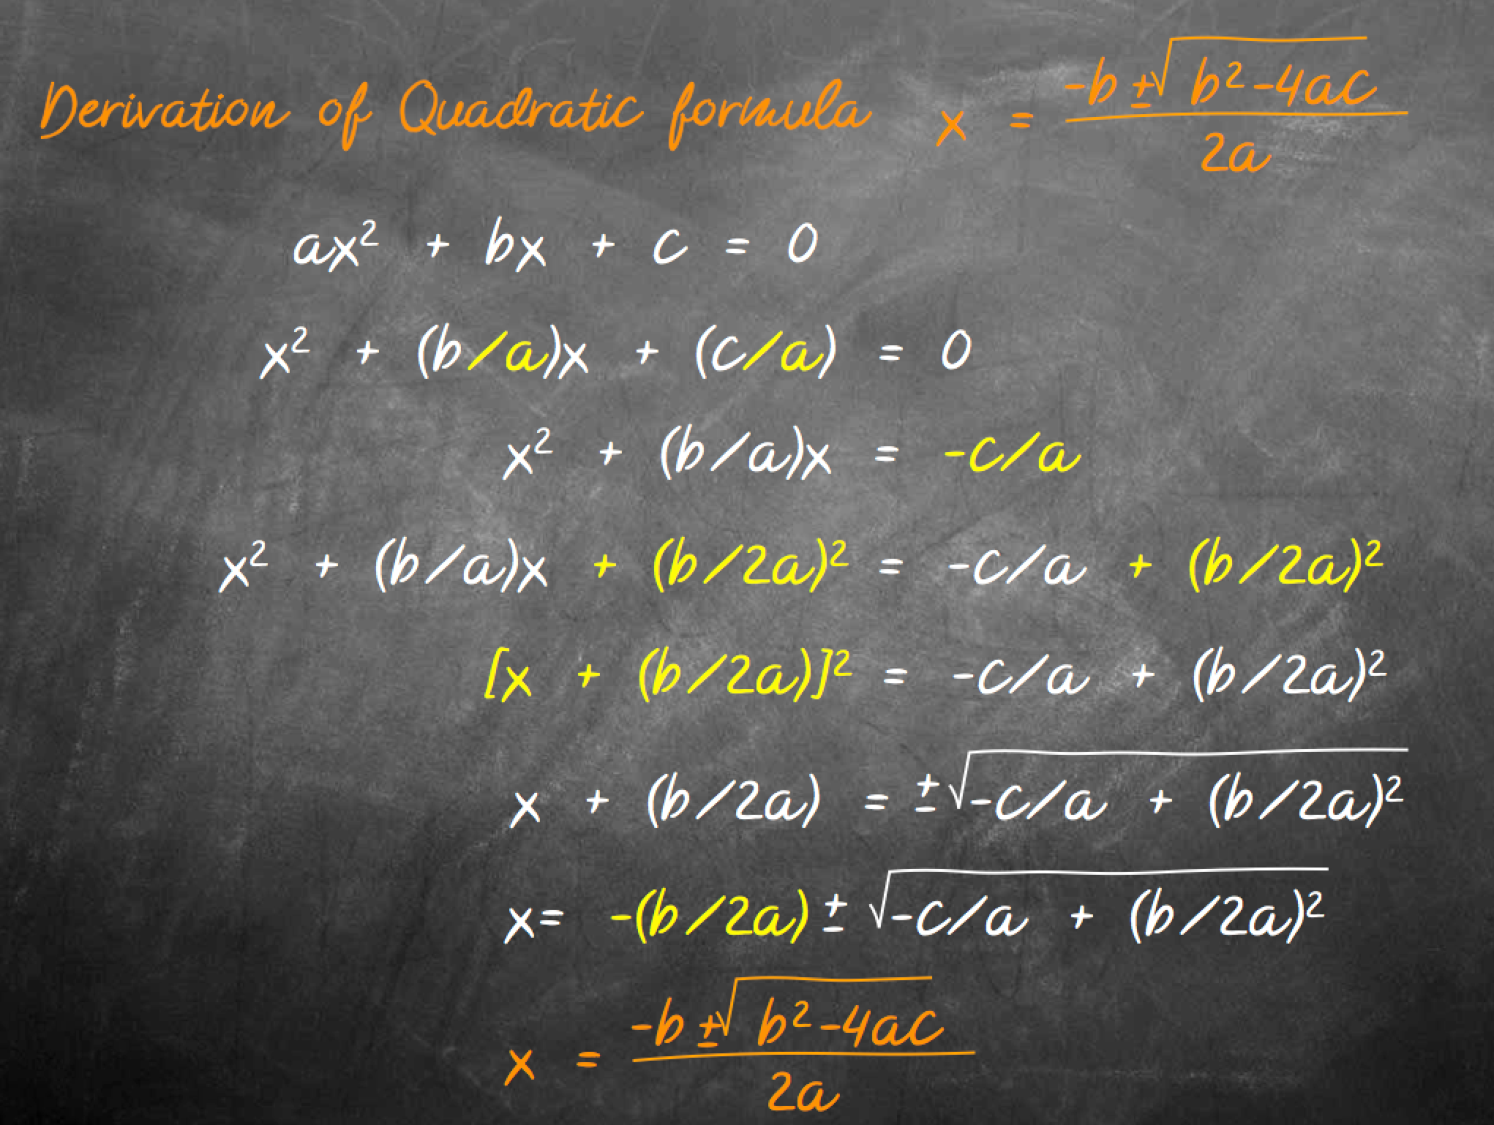
\includegraphics[width=1\columnwidth]{figures/quadformula}
        \caption{Lorem ipsum}
    \end{subfigure}  
    ~
    \begin{subfigure}[t]{0.48\columnwidth}
        \centering
        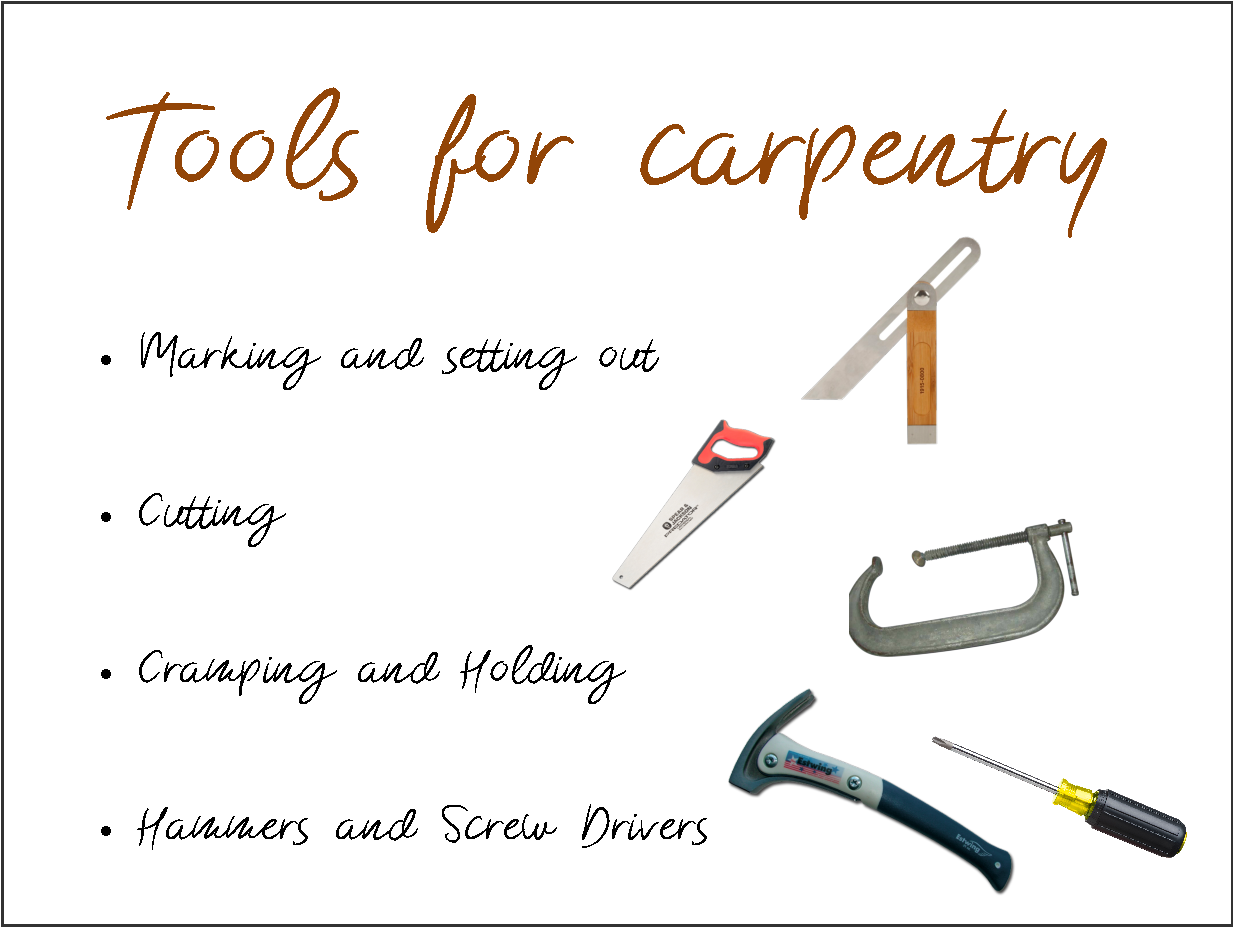
\includegraphics[width=1\columnwidth]{figures/tools}
        \caption{Lorem ipsum}
    \end{subfigure}  
    \caption{Evaluation slides}
\end{figure}

We evaluate \interface\ from two perspectives: from the presenter's point of view and from the audience's point of view. 

%\wil{If we have time, it could be useful to include even an informal
%  evaluation of the space manipulation features. Maybe just give users
%  a script that includes explicit ``improvisations'' beyond the
%  prepared content and ask for qualitative feedback?}

\val{Explain that we specifically focus on the delivery stage (vs. authoring).}
To better understand the benefits of our interface, we evaluated \interface against two baselines. The first baseline (\textit{BaselinePPT}) represents conventional electronic slides. We use Microsoft PowerPoint, and allow users to apply animation effects, but disallow inking during presentation. The second baseline (\textit{BaselineInk}) represents plain inking condition. We also use Microsoft PowerPoint, but this time we allow users to only use inking without any animations. 

We hypothesized that different types of content will lend themselves to different presentation styles. We compare three different types of content: (1) a text-centered content, explaining the derivation of the quadratic formula \textit{(Derivation)}, (2) a diagram-centered content, describing the hydrologic cycle  \textit{(WaterDiagram)}, and (3) a typical PPT style content with bullet points and images  \textit{(BulletPoints)}, listing different carpentry tools. Using PowerPoint, we pre-authored a single page slide for each of these content types, and separated the elements on each slide into foreground and background elements.  
\val{Figure of three slides, including explanation of background foreground}

\subsection{Presenter's Perspective}
For each trial, participants were given a slide and asked asked to deliver a presentation with it on one of the interfaces. They received verbal and written explanations of the slide content, and had time to familiarize themselves. They were also given time to set up the slide before the presentation. In the BaselinePPT condition, participants could set animation effects on the foreground elements. For the BaselineInk condition, the slide only contained background elements \val{Figure} and participants received a separate printed copy of the slide containing both background and foreground elements. (The printout was available for all conditions.) Participants could set up by writing contents beforehand. This is analogous to a blackboard lecturer writing on the board the before class. For \interface, participants could set up by either revealing foreground elements or writing on top of the slides ahead of time. 

To simulate a real presentation with an audience, participants were asked to pretend that their presentation was being broadcast live as a webcast. We screen recorded each presentation. At the end of each trial, we showed the recording to the presenter, and asked them to self-rate their own presentation, this time pretending that they were students trying to learn the subject. Presenters also completed a questionnaire about each interface.

We used a within-subject design, where each participant delivered presentations on each interface. We counter-balanced the order of the interfaces and the assignment of the content to interfaces. There were 12 participants in total (ages 21 to 31), all of whom were familiar with the PowerPoint interface. 

\subsection{Audience's Perspective}
We conducted a second study, where a separate set of participants were recruited to vote on the presentations delivered using each interface. Although presenters used pre-authored slides in the first study, they were not forced to follow fixed scripts. Hence, the presentations produced in the first study varied considerably in quality (e.g., length, voice, enthusiasm) depending on the presenter. To minimize the effect of the presenter, one of the authors of this paper produced a new set of presentations using the slides from the first study and following fixed scripts. To minimize author bias, we analyzed the presentations from the first study, and used them as a reference. For example, for the BaselinePPT condition, the granularity and order of animations were reproduced from what the presenters in the first study had. In the BaselineInk condition, we referenced the ordering of the inked contents and the choice of ink colors. We also recorded the presentations in such a way that the silent pauses in between inking periods were similar or shorter than in the first study. Finally, for \interface, we referenced the order of revealing, common ink annotations, and the use of slow tracing versus fast scribbling-like gestures to reveal. In most cases, presenters from the first study employed similar approaches so it was straight-forward to extract common qualities. For the few cases, where participants varied in their approach, we selected an approach that was deemed to produce better quality (e.g., finer-grained animations, use of different ink colors). The final recordings of the presentations from both studies are included in the supplementary material. 

We recruited 36 participants to rate the presentations. For each subject matter, participants watched the recordings of three presentations delivered using each interface (9 presentations in total), and voted for the most engaging presentation. 















% BALANCE COLUMNS
\balance{}

% REFERENCES FORMAT
% References must be the same font size as other body text.
\bibliographystyle{SIGCHI-Reference-Format}
\bibliography{sample}

\end{document}

%%% Local Variables:
%%% mode: latex
%%% TeX-master: t
%%% End:
